% --------------------------------------------------------------
% This is all preamble stuff that you don't have to worry about.
% Head down to where it says "Start here"
% --------------------------------------------------------------
 
\documentclass[12pt, twoside]{article}
 
\usepackage{fancyhdr}
\usepackage[margin=1in]{geometry} 
\usepackage{amsmath,amsthm,amssymb}
\usepackage{float}

\usepackage{fancyvrb, newverbs}
\usepackage{xcolor}

\usepackage{enumitem}

\usepackage{graphicx}
% -------------------------------------------------------------
% Graphics path
% -------------------------------------------------------------
\graphicspath{{../graphs/}}

% -------------------------------------------------------------
% Verbatim background
% -------------------------------------------------------------
\definecolor{verbbg}{gray}{0.93}
\newverbcommand{\cverb}
  {\setbox\verbbox\hbox\bgroup}
  {\egroup\colorbox{verbbg}{\box\verbbox}}

% -------------------------------------------------------------
% Setup constants 
% -------------------------------------------------------------
\newcommand{\name}{Ethan Febinger, Ryan Mao \\ NetIDs: eef45, rym15}
\newcommand{\class}{CS 440: Intro to AI}
\newcommand{\hwTitle}{Project 2} % Change this for a new homework
\newcommand{\due}{March 22, 2021} % Change this for a new homework


% --------------------------------------------------------------
% Setup header and footer.
% --------------------------------------------------------------
\pagestyle{fancy}
\fancyhf{}
\fancyhead[C]{\hwTitle \hfill \thepage}
\fancyfoot[C]{\name \hfill \class}
\setlength{\headheight}{14.5pt} % set head height
\renewcommand{\headrulewidth}{0.4pt} % default is 0pt
\renewcommand{\footrulewidth}{0.4pt} % default is 0pt
 
\newcommand{\N}{\mathbb{N}}
\newcommand{\Z}{\mathbb{Z}}

\newcommand\ddfrac[2]{\frac{\displaystyle #1}{\displaystyle #2}}
 
\newenvironment{theorem}[2][Theorem]{\begin{trivlist}
\item[\hskip \labelsep {\bfseries #1}\hskip \labelsep {\bfseries #2.}]}{\end{trivlist}}
\newenvironment{lemma}[2][Lemma]{\begin{trivlist}
\item[\hskip \labelsep {\bfseries #1}\hskip \labelsep {\bfseries #2.}]}{\end{trivlist}}
\newenvironment{exercise}[2][Exercise]{\begin{trivlist}
\item[\hskip \labelsep {\bfseries #1}\hskip \labelsep {\bfseries #2.}]}{\end{trivlist}}
\newenvironment{problem}[2][Problem]{\begin{trivlist}
\item[\hskip \labelsep {\bfseries #1}\hskip \labelsep {\bfseries #2.}]}{\end{trivlist}}
\newenvironment{question}[2][Question]{\begin{trivlist}
\item[\hskip \labelsep {\bfseries #1}\hskip \labelsep {\bfseries #2.}]}{\end{trivlist}}
\newenvironment{corollary}[2][Corollary]{\begin{trivlist}
\item[\hskip \labelsep {\bfseries #1}\hskip \labelsep {\bfseries #2.}]}{\end{trivlist}}
 
\begin{document}
 
% --------------------------------------------------------------
%                         Start here
% --------------------------------------------------------------
 
\title{\hwTitle} % replace X with the appropriate number
\author{\name\\  % replace with your name
\class} % if necessary, replace with your course title
\date{\due}
 
\maketitle

\section*{Integrity}

We, Ryan Mao and Ethan Febinger, certify that the code and report for this assignment are our work alone.

\section*{Work Division}

    Ryan Mao: Problems 1-4, 6 

    \noindent Ethan Febinger: Problems 5, 7, 8


\tableofcontents
\vfill
\pagebreak
\section{Writeup}
\begin{enumerate}[itemsep=2mm,parsep=4mm]
    \item 
        \textit{Representation: How did you represent the board in your program, and how did you represent the information/knowledge that clue cells reveal? How could you represent inferred relationships between cells?}
    
        The board was simply represented as a 2D matrix of cells. In this, each cell can be one of three things. If the cell is covered (i.e. the user/agent has not decided to query this cell), there will be a `?' at the corresponding location. If the cell has been queried before and is a mine, there will be a `M' present. If the cell has been queried and is safe (i.e. the cell itself is NOT a mine), there will be the appropriate clue value which describes the number of mines directly surrounding the current cell. 

        The knowledgebase consists of four 2D matrices. The first 2D matrix is the current board using the same representation methods discussed above. The second 2D matrix is the number of safe (non-mine) squares around a given cell. For example, if there are 2 mines around a cell with indices (i, j), then at indices (i, j) for this 2D matrix will be 6, as there are 6 cells around the current cell that are not mines. Our third 2D matrix in our knowledgebase is precisely the negation of the second 2D matrix. Examining the same cell as in the previous example, at indices (i, j) for the third 2D matrix would be a 2. Lastly, the fourth 2D matrix stores the amount of covered/unqueried cells around a current cell.

        The inferred relationships between cells is represented as sets. For example, if a cell has a clue value of 2, and none of the uncovered cells next to it are mines, then we know that the set of cells around the current cell has 2 mines in it. So, we say that $C = \{\text{number of nearby covered cells}\}$ and this has a value of $2$. We then know any subset, $A$, of this set has to have a value say $v$, which is $\leq 2$. Thus, the $C - A = 2 - v$. From this, we can perform a sort of induction to aid our agent in the minesweeper program.

    \item 
        \textit{Inference: When you collect a new clue, how do you model/process/compute the information you gain from it? In other words, how do you update your current state of knowledge based on that clue? Does your program deduce everything it can from a given clue before continuing? If so, how can you be sure of this, and if not, how could you consider improving it?}
    
    \item 
        \textit{Decisions: Given a current state of the board, and a state of knowledge about the board, how does  your program decide which cell to search next?}

    \item 
        \textit{Performance: For a reasonably-sized board and a reasonable number of mines, include a play-by-play progression to completion or loss. Are there any points where your program makes a decision that you don’t agree with? Are there any points where your program made a decision that surprised you?  Why was your program able to make that decision?}

    \item 
        \textit{Performance: For a fixed, reasonable size of board, plot as a function of mine density the average final score (safely identified mines / total mines) for the simple baseline algorithm and your algorithm for comparison. This will require solving multiple random boards at a given density of mines to get good average score results. Does the graph make sense / agree with your intuition? When does minesweeper become ‘hard’? When does your algorithm beat the simple algorithm, and when is the simple algorithm better? Why? How frequently is your algorithm able to work out things that the basic agent cannot?}

        For both the basic algorithm and the advanced algorithm, we use a dimension size of 25, so the minesweeper board is a 25 by 25 square board.

        \begin{figure}[H]
            \centering
            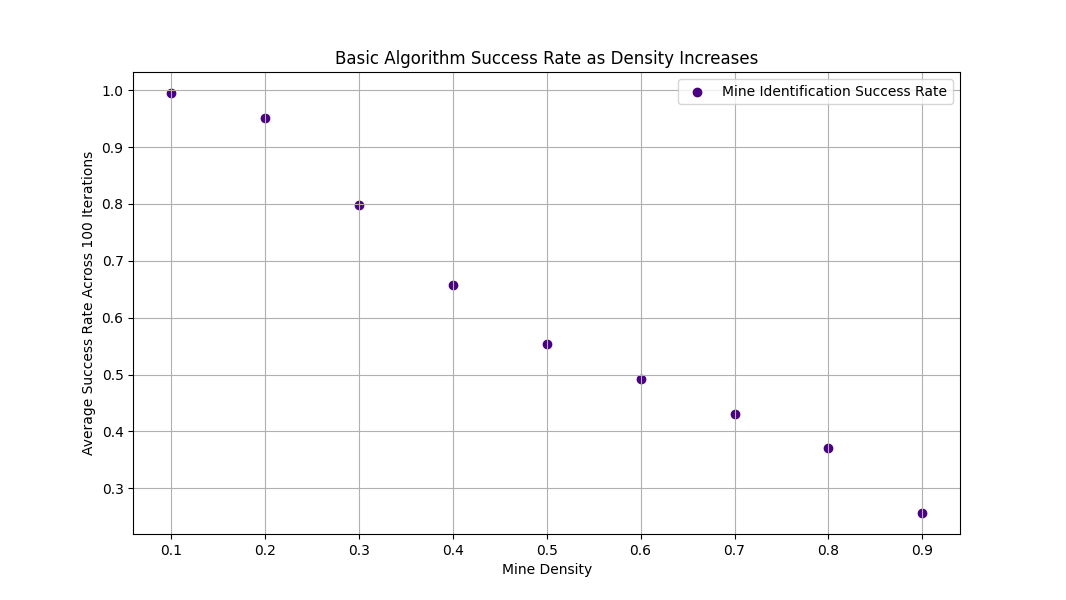
\includegraphics[scale = 0.55]{Basic Algorithm.png}
        \end{figure}
        \begin{figure}[H]
            \centering
            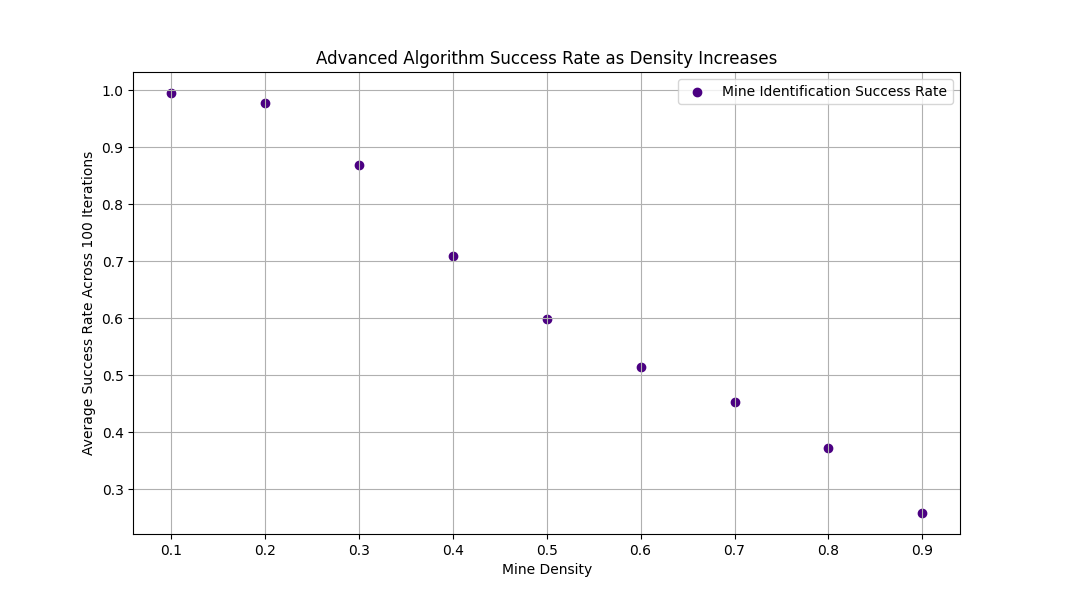
\includegraphics[scale = 0.55]{Advanced Algorithm.png}
        \end{figure}

        We can see that the advanced algorithm slightly outperforms the basic algorithm up until around a mine density of 0.8, where both algorithms obtain the same success results.

        This makes sense for the advanced algorithm to do slightly better than the basic algorithm, as it is performing more induction, and attempting to `reason' using logic and finding contradictions.

        Minesweeper becomes `hard' for both algorithms at around \textbf{INSERT VALUE}.

        There is not a time where the simple algorithm is better. The advanced algorithm is either better by a small margin, or the same. This liens up with our prediction/algorithm since the advanced algorithm performs the basic algorithm logic until it has to guess. Then it attempts to deduce something by assuming certain cells to be a mine. Depending on whether or not the algorithm then reaches a contradiction, the algorithm can slowly rule out certain cells as mines. If it is unable to deduce anything more, however, it will then make another guess.
    \item 
        \textit{Efficiency: What are some of the space or time constraints you run into in implementing this program? Are these problem specific constraints, or implementation specific constraints? In the case of implementation constraints, what could you improve on?}

\end{enumerate}
 
\vfill
\pagebreak
\section{Non-Standard Libraries Used}

\begin{enumerate}
    \item
        \textit{matplotlib} - Generating and saving graphs.
    \item
        \textit{numpy} - arange function to generate equally separated float values between two floats.
        Was also used for generating curves of best fit, but is omitted from the submitted code.
\end{enumerate}
% --------------------------------------------------------------
%     You don't have to mess with anything below this line.
% --------------------------------------------------------------
 
\end{document}